\documentclass[unicode,aspectratio=169,11pt]{beamer}
\usepackage{amsmath, amssymb, amsthm, color, latexsym, mathrsfs, bm}
\usefonttheme{professionalfonts}
\usepackage{luatexja}
\usepackage[ipaex]{luatexja-preset}
\renewcommand{\kanjifamilydefault}{\gtdefault}

\usetheme[
  sectionpage=none,
  numbering=fraction,
  block=fill
  ]{metropolis}

\title{
    The AI economist:
    Improving Equality and Productivity with AI-Driven Tax Policies
}
\subtitle{Stephan Zheng, Alexander Trott, Sunil Srinivasa, Nikhil Naik, Melvin Gruesbeck, David C. Parkes, and Richard Socher, 2020, mimeo.}
\author{発表者: 冨田 燿志}
\date{2021年6月21日 PaperFriday}

\begin{document}

\maketitle

\section{1. イントロダクション}
\begin{frame}{1. イントロダクション}
    \begin{itemize}
        \item 最適な課税・再分配制度のデザインは重要だが難しい問題である.
        \item その難しさの一因は, 生産性と平等性のトレードオフ:
        \begin{itemize}
            \item 税を低くすると, 経済行動が活発になり生産性は増すが不平等になる.
            \item 税を高く再分配を厚くすると, 経済行動が抑制され生産性が落ちる.
        \end{itemize}
         \\
        \item 最適課税理論の分野で研究が進むが, 明確な答えは得られていない:
        \begin{itemize}
            \item 税率変化の経済行動への影響(弾力性)の推定が困難.
            \item 税制をフィールド実験することはほぼ不可能.
        \end{itemize}
         \\
        \item この論文では, 経済シミュレーションゲームにおいて, 政府主体に最適な税制を深層強化学習により学習させることを考える(AI Economist).
        \item 市民をRLエージェントとするシミュレーション実験と, 人を被験者とする実験の双方で, AI economist による税制は生産性・平等性のトレードオフを高い水準で達成した.
    \end{itemize}
\end{frame}

\section{2. Gather-and-Build Games}

% \begin{frame}{2. Economic Simulations: Learning in Gather-and-Build Games}{}
%     \begin{itemize}
%         \item Economic environmentについて.
%         \item まずは税の無い設定("free-market")で説明する.
%     \end{itemize}
% \end{frame}

% \subsection{2.1 Notation and Preliminaries}
% \begin{frame}{2.1 Notation and Preliminaries}
%     \begin{itemize}
%         \item Partial-observable multi-agent Markov Games(MGs): $(S, A, r, \mathscr{T}, \gamma, o, \mathscr{I})$
%         \begin{itemize}
%             \item $S$ : 状態空間(state space)
%             \item $A$ : 行動空間(action space)
%             \item $r_{i,t}$ : 報酬関数(reward function)
%             \item $\mathscr{T}$ : 遷移関数(transition function)  $s_{t+1} \sim \mathscr{T}(\cdot \mid s_t, \bm{a}_t)$
%             \item $\gamma$ : 割引因子(discount factor)
%             \item $o_{i,t}$ : 観測(observation)
%             \item time step $t = 0, 1, \dots, H$.
%         \end{itemize}
%     \end{itemize}
% \end{frame}

% \begin{frame}{}{}
% \begin{itemize}
%     \item Agents' policy : $\pi_i(\cdot \mid o_{i,t}, h_{i,t}; \theta_i)$
%     \begin{itemize}
%         \item $h_{i,t}$ : hidden state(自分の私的情報と, 過去のhistory)
%         \item $\theta_i$ : policyのparameter
%         \item エージェント $i$ は次の最大化問題を得くpolicyを求める:
%         \[
%             \max_{\theta_i} \mathbb{E}_{a_i \sim \pi_i, \bm{a}_{-i} \sim \bm{\pi}_{-i}, s'\sim \mathscr{T}}\left[\sum_{t}\gamma^t r_{i,t}\right].
%             \tag{1}
%         \]
%     \end{itemize}
%      
%     \item データ効率性のため, すべてのエージェントはtrainingの間パラメータ$\theta$を共有する.
%     \item 彼らの行動 $\pi_i(a_i\mid o_i, h_i; \theta)$ は, agent-specific observations $o_i$ と hidden-state $h_i$によって異なる.
% \end{itemize}
% \end{frame}

% \begin{frame}
%     \begin{center}
%         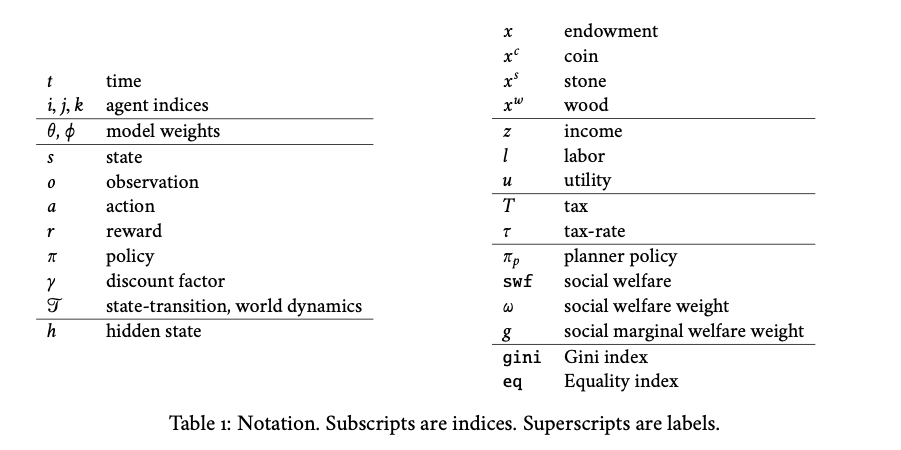
\includegraphics[width=15cm]{table1.png}
%     \end{center}
% \end{frame}

\begin{frame}{2. Gather-and-Build Games}{}
{\bf Gather-and-Build game(収集建築ゲーム)}
\begin{itemize}
    \item 2次元のグリッド ($25 \times 25$) からなる世界が舞台.
    \item 市民はフィールドを歩き回り, 資源(石と木)を集め, それらを1つずつ使って家を建てコインを稼ぎ, またコインを介して資源の取引をする.
    \item 資源は空タイルに確率的に産み出される.
    \item 市民は家を建てるとコインが得られるが, 得られるコインの数は各市民のスキルごとに異なる.
    \item (政府主体・税制度は後述)
\end{itemize}
\end{frame}

\begin{frame}{}{}
{\bf 労働とスキル.}
\begin{itemize}
    \item 市民の行動(移動, 収集, 取引, 建築)にはそれぞれ労働コストが設定されている.
    \item 各期に市民がどれか1つの行動をとると, 設定されている労働コストがかかる.\\
     
    \item 建築には, 木と石の資源が1つずつ必要.
    \item 建築スキル(1以上3以下)が各市民に設定されていて, 建築をすると市民は $10\ \times$ スキル 枚のコインを得る.\\
     
\end{itemize}
{\bf 取引.}
\begin{itemize}
    \item 取引を選択した市民は, 市場に売り注文「コインX枚以上で木を売ります」か, 買い注文「コインY枚以下で石を買います」を送る.
    \item 市場に売り注文買い注文が出れば, 先に注文を出した側の値段で自動的に取引がされる.
        \begin{itemize}
            \item 複数ある場合はより条件の良い注文が優先される.
            \item 一定期間取引相手が見つからなかった注文は市場から削除される.
        \end{itemize}
\end{itemize}
\end{frame}

\begin{frame}{}{}
\begin{columns}[t]
    \begin{column}{0.6\textwidth}
        {\bf シナリオ.}
        \begin{itemize}
            \item フィールドは水により4つの区域に別れている(水部分は通れない)
            \item 資源は空間的に集まって発生する.
            \item 市民は4人.
            \item 建築スキルは 1.13, 1.33, 1.65, 22.2 で固定(パレート分布の分位点を元に設定)
            \item 1エピソードは, $1000$ステップからなる.
            \item 市民は自身の位置の近く($11\times11$)のみの状況が観測できる.
        \end{itemize}
    \end{column}
    \begin{column}{0.4\textwidth}
        \begin{center}
            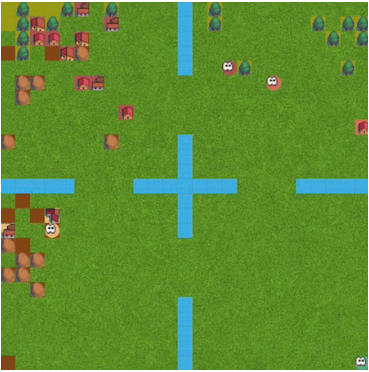
\includegraphics[width=5cm]{figure1.png}
        \end{center}
    \end{column}
\end{columns}
\end{frame}

\begin{frame}{2.1 市民の最適化行動}{}
    \begin{itemize}
        \item 市民の効用関数:
        \[
            u_i(x_{i,t}, l_{i,t}) = \frac{(x_{i,t}^{c})^{1-\eta} - 1}{1-\eta} - l_{i,t}.
            \tag{2}
        \]
        \begin{itemize}
            \item $x_{i,t} = (x_{i,t}^w, x_{i,t}^s, x_{i,t}^c)$: 市民$i$が$t$期時点で保有する木・石・コイン.
            \item $l_{i,t}$: $t$期までの蓄積労働量.
            \item $\eta \in (0, 1)$: 市民の効用関数の非線形性をコントロールするパラメータ.
        \end{itemize}
        \item 合理的な市民は以下の最大化を行う.
        \[
            \forall i : \max_{\pi_i} \mathbb{E}_{a_i \sim \pi_i,\ \bm{a}_{-i}\sim \bm{\pi}_{-i}, s'\sim \mathscr{T}}
            \left[u_i(x_{i,0}, l_{i,0}) + \sum_{t=1}^H\gamma^t \underbrace{\left(u_i(x_{i,t}, l_{i,t})-u_i(x_{i,t-1}, l_{i,t-1})\right)}_{=r_{i,t}}\right].
            \tag{3}
        \]
        \begin{itemize}
            \item $\pi_i$: 状態 $s \in \mathscr{T}$ と観測 $o_{i,t}$ から行動 $a_{i,t}$ を選ぶポリシー
            \item $\gamma \in (0, 1)$: 割引因子
        \end{itemize}
    \end{itemize}
\end{frame}

\begin{frame}{}{}
{\bf 深層強化学習エージェント}
\begin{itemize}
    \item ディープニューラルネットワークを用いて市民のポリシーをモデリングする:
    \[ a_{i,t} \sim \pi(o^{\mathrm{world}}_{i,t}, o^{\mathrm{agent}}_{i,t}, o^{\mathrm{market}}_{i,t}, o^{\mathrm{tax}}_{i,t}, h_{i,t-1};\theta) \]
    \begin{itemize}
        \item $o^{\mathrm{world}}_{i,t}$: 近くの状況に関する観測.
        \item $o^{\mathrm{agent}}_{i,t}$: 市民の状況(資源・コイン保有)
        \item $o^{\mathrm{market}}_{i,t}$: 市場の状況(売り注文・買い注文の蓄積状況)
        \item $o^{\mathrm{tax}}_{i,t}$: 税率(後述)
        \item $h_{i, t-1}$: hidden state(自身のプライベートな状況(スキルと労働蓄積量)と過去の履歴)
        \item $\theta$: モデルのパラメータ
    \end{itemize}
\end{itemize}
\end{frame}

\begin{frame}{}{}
    \begin{center}
        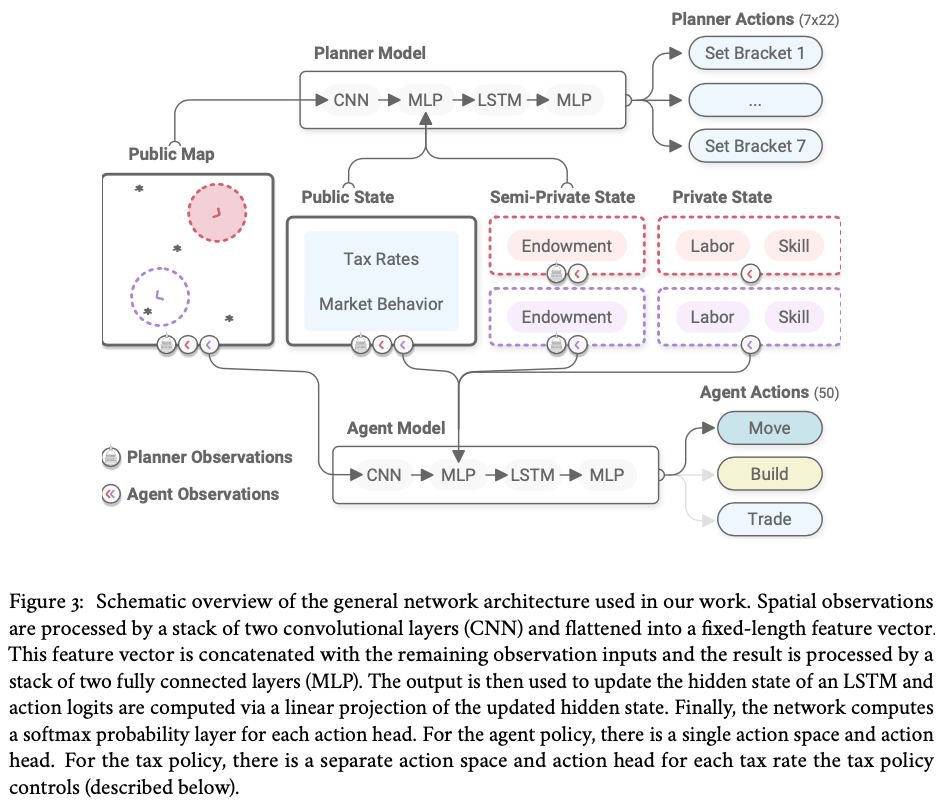
\includegraphics[width=10.3cm]{figure3.png}
    \end{center}
\end{frame}

\begin{frame}{}{}
    {\bf 無課税・無分配下での市民の行動}
\begin{columns}[t]
    \begin{column}[]{0.6\textwidth}
        \begin{center}
            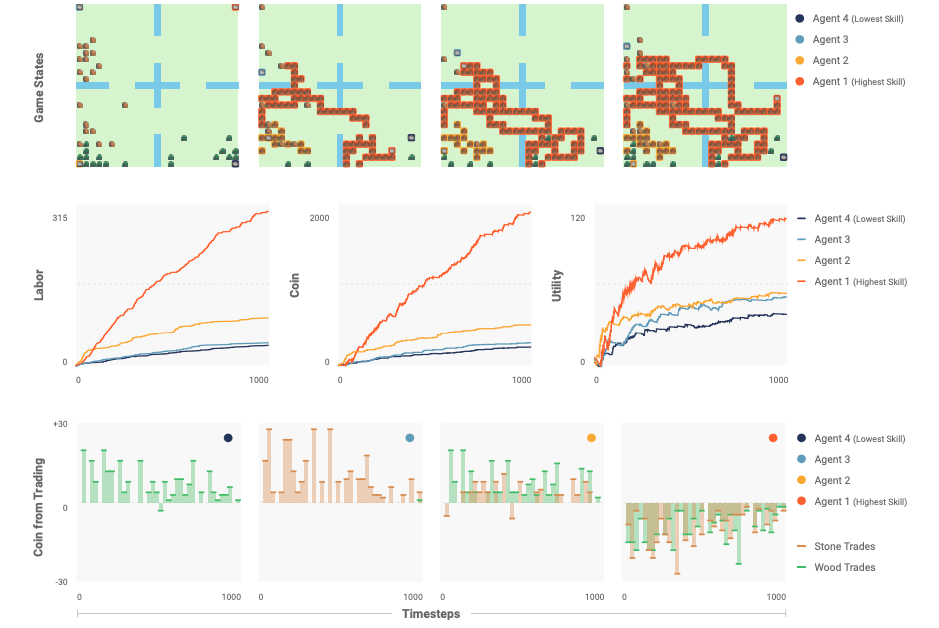
\includegraphics[width=9cm]{figure4.png}
        \end{center}
    \end{column}
    \begin{column}[]{0.4\textwidth}
        \begin{itemize}
            \item 左図は無課税下で学習後の各市民の1エピソードの行動.
            \item 低スキル市民(紺,水)は資源を集めて市場で売ることに徹している.
            \item 高スキル市民(オレンジ)は市場で資源を買い, 自身で建築してコインを稼ぐ.
            \item 黄色は最初は建築しているが, のちに資源を売る方にスイッチしている.
        \end{itemize}
    \end{column}
    
\end{columns}
\end{frame}

\section{3. 最適課税政策の学習}
\begin{frame}{3. 最適課税政策の学習}
    \begin{itemize}
        \item 課税と再分配(のみ)を行う政府主体を導入する.
        \item 政府は, 生産性と平等性のトレードオフに直面している.
        \begin{itemize}
            \item 無課税・無分配では生産性は最大化されるが, 不平等が生まれる.
            \item 課税・再分配を行うと平等性が増すが, 生産性が落ちる.
        \end{itemize}
         \\
        \item ここでは, 無課税, 米連邦所得税, Saezフレームワーク, AI economist の4つの税制度を試す.
    \end{itemize}
\end{frame}

\subsection{3.1 税制度}
\begin{frame}{3.1 税制度}{}
{\bf 税ピリオドと再分配.}
    \begin{itemize}
        \item 税ピリオドは $M$ ステップ続く(実験では$M = 100$とし, 1エピソードに10ピリオドある)
        \item ピリオド $p$ の税は, 期初 $t$ から 期末$t + M$ までの収入 $z_i^p$ に課される.\\
                 
        \item ピリオドの初めに, 政府は税額関数 $T(z)$ を決めて公表する.
        \begin{itemize}
            \item 各市民 $i$ は, 収入 $z_i^p$ に応じて $T(z_i^p)$ を支払う.
            \item 集められた税は, 全市民に平等に分配される.
            \item よって再分配後の市民 $i$ の収入は,
            \[ \tilde{z}_i^p = z_i^p - T(z_i^p) + \frac{1}{N}\sum_{j=1}^N T\left(z_j^p\right) \tag{5}\]
            となる.
        \end{itemize}
    \end{itemize}
\end{frame}

\begin{frame}{}{}
{\bf 税ブラケット.}
\begin{itemize}
    \item 税額関数は, 次のように「ブラケット化」されたもののみを考える.
    \item カットオフ $\{m_b\}_{b = 0}^B$ s.t. $0 = m_0 \le m_1 \le \dots \le m_{B-1}\le m_B = +\infty$ が先に与えられる.
    \item 政府は, 各ブラケット $b$ に含まれる収入に対して適用される限界税率 $\tau_b \in [0,1]$を選ぶことで, 税額 $T(\cdot)$ を決定する.
    \[ T(z) = \sum_{b = 0}^{B-1} \tau_b \cdot \left((m_{b+1}-m_{b}) \cdot 1[z > m_{b+1}] + (z - m_b)\cdot 1[m_b < z \le m_{b+1}]\right).\]
    \item 例:
    \begin{itemize}
        \item カットオフ: $m_0 = 0,\ m_1 = 100, m_2 = 200, m_3 = 300, m_4 = +\infty$.
        \item 限界税率: $\tau_0 = 0.1,\ \tau_1 = 0.2,\ \tau_2 = 0.3,\ \tau_3 = 0.4$.
        \item 収入: $z_i^p = 250$
        \item 最初の$100$には税率$0.1$, 次の$100$には税率$0.2$, 次の$50$には税率$0.3$がかかるので,
        \[ T(z_i^p) = 100 \times 0.1 + 100 \times 0.2 + 50 \times 0.3 = 45. \]
    \end{itemize}
\end{itemize}
\end{frame}

\begin{frame}{3.2 政府}{}
{\bf 社会厚生関数}
\begin{itemize}
    \item 政府の目的関数である社会厚生関数は, 生産性と平等性のトレードオフを組み込めるように次のように決める.
    \item エージェントのコイン保有 $\bm{x}^c = (x_1^c, \dots, x_N^c)$ に対し, 平等性を次で定義:
    \[ {\bf{eq}}(\bm{x}^c) = 1 - {\bf{gini}}(\bm{x}^c)\cdot \frac{N}{N-1},\ \ \ 0 \le {\bf eq}(\bm{x}^c)\le 1.\tag{7} \]
    where
    \[ {\bf{gini}}(\bm{x}^c) = \frac{\sum_{i=1}^N\sum_{j=1}^N |x_{i}^c - x_{j}^c|}{2N \sum_{i=1}^N x_{i}^c},
    \ \ \ 0 \le {\bf gini}(\bm{x}^c) \le \frac{N-1}{N}\tag{8} \]
    \begin{itemize}
        \item ${\bf eq}$は, $1$で完全に平等(全員同じ収入), $0$で完全に不平等(1人が全コインを独占).
    \end{itemize}
\end{itemize}
\end{frame}

\begin{frame}{}{}
    \begin{itemize}
        \item 生産性は, 
        \[ {\bf prod}(\bm{x}^c) = \sum_{i=1}^N x_{i}^c. \tag{9} \]
        \item この平等性 ${\bf eq}$ と生産性 ${\bf prod}$ の積を社会厚生関数とする.%\footnote{Social welfare functionとして, weight $\omega_i \ge 0$ を用いて
        % \[ {\bf swf}_t(\bm{x}_t^c, \bm{l}_t) = \sum_{i = 1}^N \omega_i \cdot u_i\left(x_{i,t}^c, l_{i,t}\right). \tag{11}\]
        % を用いることも可能.}
        \[ {\bf swf}_t(\bm{x}_t^c) = {\bf eq}_t(\bm{x}_t^c) \cdot {\bf prod}_t (\bm{x}_t^c). \tag{10}\]
    \end{itemize}
\end{frame}

\begin{frame}{}{}
{\bf 政府の問題.}
\begin{itemize}
    \item 政府は,
    \begin{itemize}
        \item 市民の保有資源・コイン $\bm{x}_{i,t}$, フィールドの状態(市民・資源の位置)と取引市場の状況は観測可能,
        \item 各市民のスキル・蓄積労働コストは直接には観測できない.
    \end{itemize}
    \item 政府の最大化問題は,
    \[ \max_{\pi_p} \mathbb{E}_{\tau \sim \pi_p, \bm{a} \sim \bm{\pi}, s'\sim \mathscr{T}}\left[{\bf swf}_0+\sum_{t=1}^H\gamma^t\underbrace{({\bf swf}_t-{\bf swf}_{t-1})}_{=r_{p,t}}\right]. \tag{12} \]
\end{itemize}
\end{frame}

\subsection{3.3 Inner-Outer-Loop Reinforcement Learning}
\begin{frame}{3.3 Inner-Outer-Loop Reinforcement Learning}{}
    \begin{columns}[t]
        \begin{column}[]{0.6\textwidth}
            \begin{center}
                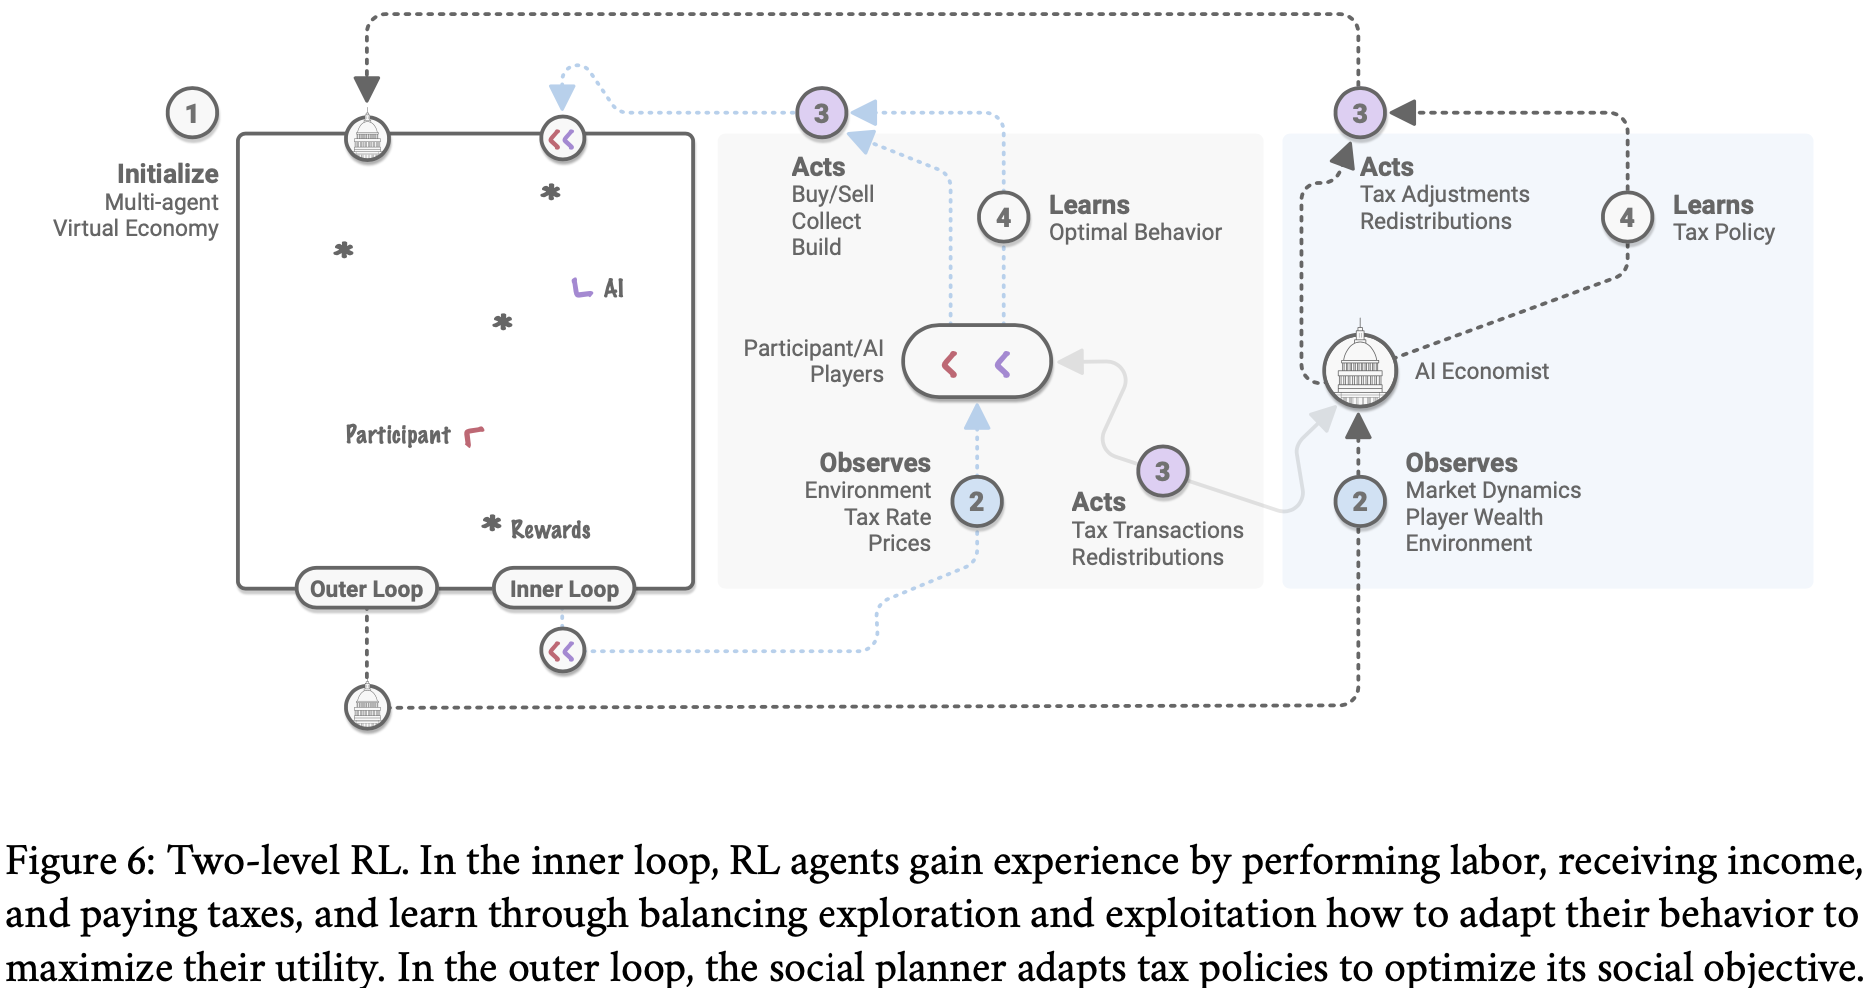
\includegraphics[width=9cm]{figure6.png}
            \end{center}
        \end{column}
        \begin{column}[]{0.4\textwidth}
            \begin{itemize}
                \item この状況では, 内側のループで市民が行動を選んで学習し, 外側のループで政府が税制を選んで学習することになる.
                \item 市民の学習行動と政府の選ぶ税制が相互に影響し合うため, 報酬が不安定になり, 初期の学習に工夫が必要.
            \end{itemize}
        \end{column}
    \end{columns}
\end{frame}

% \begin{frame}
%     \begin{center}
%         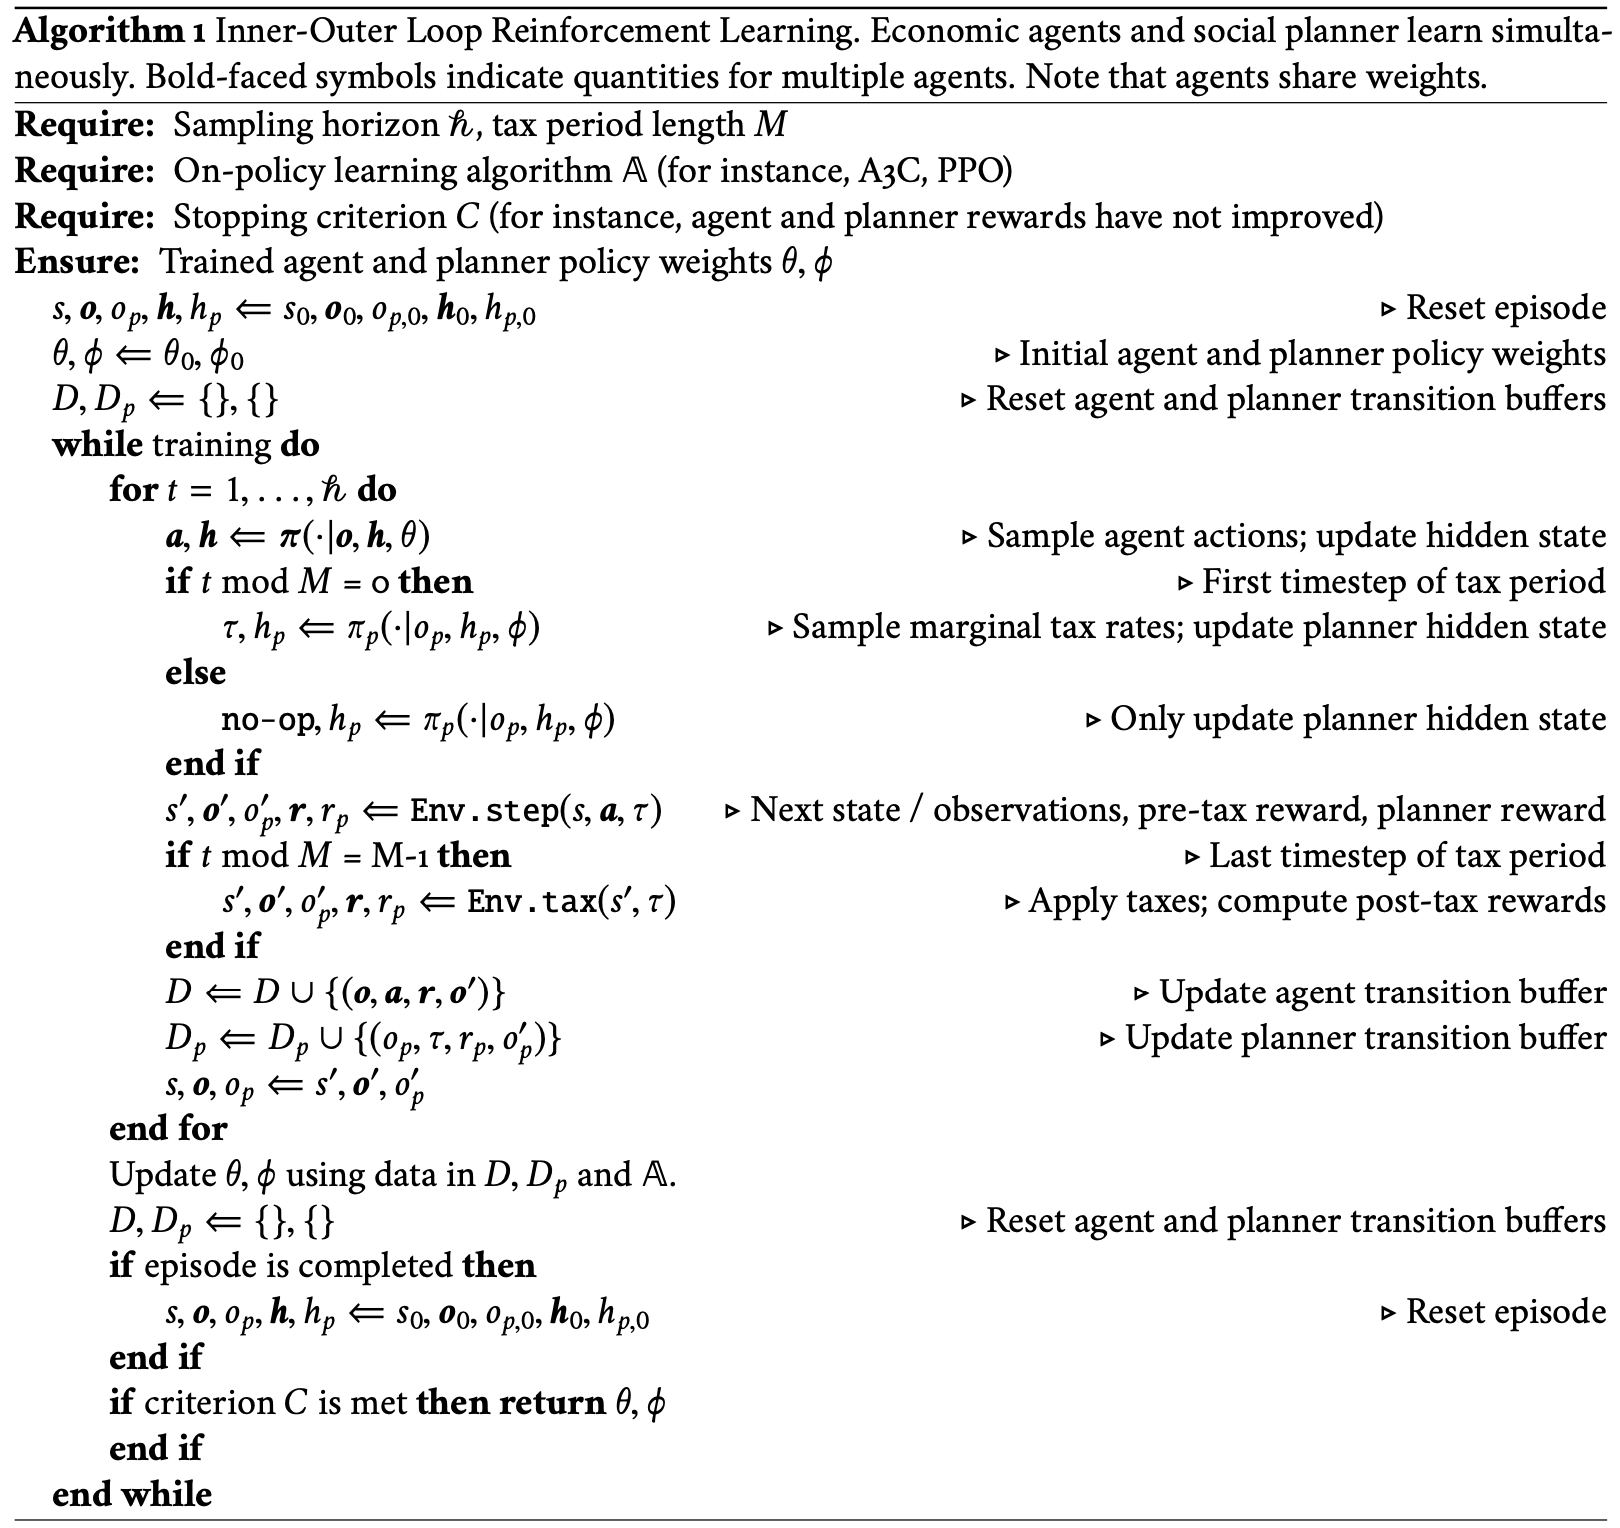
\includegraphics[width=9.3cm]{algorithm1.png}
%     \end{center}
% \end{frame}

\section{4. AI市民実験}
\begin{frame}{4. AI市民実験}{}
{\large\bf 4.1 ベースライン}
\begin{itemize}
    \item 次の4つの税制度を比較する.
    \begin{itemize}
        \item 無課税(フリーマーケット)
        \item 2018米連邦所得税
        \item Saezフレームワーク
        \item AI Economist
    \end{itemize}
    \item ブラケットは全ての税制に共通で, 2018年米所得税をもとに1/1000にスケーリングしたものを用いる.
    \[ \bm{m} = [0, 9.7, 39.475, 84.2, 160.725, 204.100, 510.3, \infty]. \tag{15} \]
\end{itemize}
\end{frame}

\begin{frame}{}{}
{\bf 2018米連邦所得税.}
\begin{itemize}
    \item 2018年の米連邦所得税をもとに, 各ブラケットの税率は, 
    \[ \bm{\tau} = [0.1, 0.12, 0.22, 0.24, 0.32, 0.35, 0.37] \tag{16} \]
    とする.
\end{itemize}    
\end{frame}

\begin{frame}{}{}
{\bf Saez Tax Formula (single-period)}
\begin{itemize}
    \item Saez [2001]をもとに, まずsingle-period economyでのoptimal tax ratesを求める.
    \item $f, F$は(pre-tax)収入の分布のprobability densityとcummulative distribution functionとし, plannerはそれらを観測できるとする.
    \item Saez [2001]では, まずlinear-weighted social welfare functions (11)に対し, social marginal welfare weights
    \[ g_i = \frac{\mathrm{d}{\bf swf}}{\mathrm{d} u_i} \frac{\mathrm{d} u_i}{\mathrm{d} x_{i}^c} = \omega_i \frac{\mathrm{d} u_i}{\mathrm{d} x_{i}^c}.  \]
    を求める.
    \item これを我々のモデルに当てはめるために$g_i = \frac{1}{z_i}$とし, さらにこれをnormalizeしてよい $\sum_{i \in \mathscr{T}}g_i = 1$.
\end{itemize}
\end{frame}

\begin{frame}{}{}
    \begin{itemize}
        \item $\alpha(z)$を, the marginal average income at income z, normalized by the fraction of incomes above z, つまり,
        \[ \alpha(z) := \frac{z \cdot f(z)}{1 - F(z)}. \tag{18}\]
        \item $G(z)$は, normalized, reverse cumulative Pareto weight over incomes above a threshold z
        \[ G(z) := \frac{1}{1 - F(z)}\int_{z' = z}^\infty f(z')g(z') \mathrm{d}z'. \tag{19}\]
        \item また, 弾力性(elasticity) $e(z)$を, average sensitivity of an agent’s income to changes in the tax rate, つまり
        \[e(z) = \frac{\mathrm{d}z / z}{\mathrm{d}(1 - \tau(z))/(1-\tau(z))}. \tag{20}\]
        \item Saez [2001]によると, optimal marginal tax-rateは
        \[ \tau(z) = \frac{1 - G(z)}{1 - G(z) + \alpha(z) e(z)} \tag{21}\]
        となり, これはincome distributionとelasticityに依存して決まる.
    \end{itemize}
\end{frame}

\begin{frame}{}{}
{\bf Saez Tax Formula (multi-period)}
\begin{itemize}
    \item Saez formula (21) を使うには, income elasticity $e(z)$ の推定が必要.
    \item Gruber and Saez [2002]に従い, constant tax elasticity $\tilde{e}$ を仮定すると, 
    \[ z_t = z^0 \cdot (1- \tau_t)^{\tilde{e}}. \tag{22} \]
    \item したがって, 
    \[ \log(z_t) = \tilde{e} \cdot \log(1 - \tau_t) + \log(z^0) \tag{23} \]
    を過去のtax periodのデータからOLSで推定して用いる.
\end{itemize}
\end{frame}

\begin{frame}{}{}
    \begin{itemize}
        \item AI Economistは, ディープニューラルネットワークにより各ブラケットの限界税率を決める.
        \[ \tau \sim \pi_p\left( o^{\mathrm{world}}_{p,t}, o^{\mathrm{agent}}_{p,t}, o^{\mathrm{market}}_{p,t}, o^{\mathrm{tax}}_{p,t}, h_{p, t-1} ; \phi \right). \tag{24} \]
        \begin{itemize}
            \item 基本のネットワークアーキテクチャは市民と同様(Figure 3).
            \item 市民と政府は観測できるものが異なる(政府はフィールド全体が見れるが, 市民のスキルは見れない).
        \end{itemize}
    \end{itemize}
\end{frame}

\subsection{4.2 Training Strategy: Two-phase Training and Tax Curricula}
\begin{frame}{4.2 Training Strategy: Two-phase Training and Tax Curricula}
\begin{itemize}
    \item Section 3.3で述べたように, このjoint optimizationは不安定性をもたらす.
    \item 学習を安定化させるため, ここでは次のtwo-pahse training approachを行った.
    \begin{itemize}
        \item First phaze: agent modelsの集合に対し, 無課税(no-tax scenario)で学習させる.
        \item Second phaze: 税モデルを融合にし, エージェント・プランナーの学習を継続する.\\
                また突然の税導入による不安定性を回避するため, 限界税率の上限を$10\%$から$100\%$に徐々に引き上げる.
    \end{itemize}
    \item また, planner policyにentropy regularizationを行うことも効果的だった.
    \begin{itemize}
        \item Entropy regularizationは, policy gradient objectiveに次のadditional, weighted term
        \[ {\bf entropy}(\pi) = - \mathbb{E}_{a \sim \pi(\cdot \mid s)} [\log\pi(a \mid s)]. \]
        を加える(Williams and Peng [1991], Mnih et al. [2016]).
    \end{itemize}
\end{itemize}
\end{frame}

\begin{frame}{}{}
\begin{itemize}
    \item 実験はRLlib flamework [Liang et al., 2018]を用いて実施.
    \item またPolicy gradientsの計算に, proximal policy gradients [Schulman et al., 2017]とAdam optimizer [Kingma and Ba, 2014] を使う.
    \item サンプルは60のenvironment replicasから平行して集め, sampling horizonは200 timestepsとする.
    \item 全ての実験で, 400 million sampleのphase two trainingを実施し, これはagentとplanner modelはstable policyへの収束に十分であった.
\end{itemize}
\end{frame}

\subsection{4.3 平等性, 生産性と社会厚生}
\begin{frame}{4.3 平等性, 生産性と社会厚生}{}
    \begin{center}
        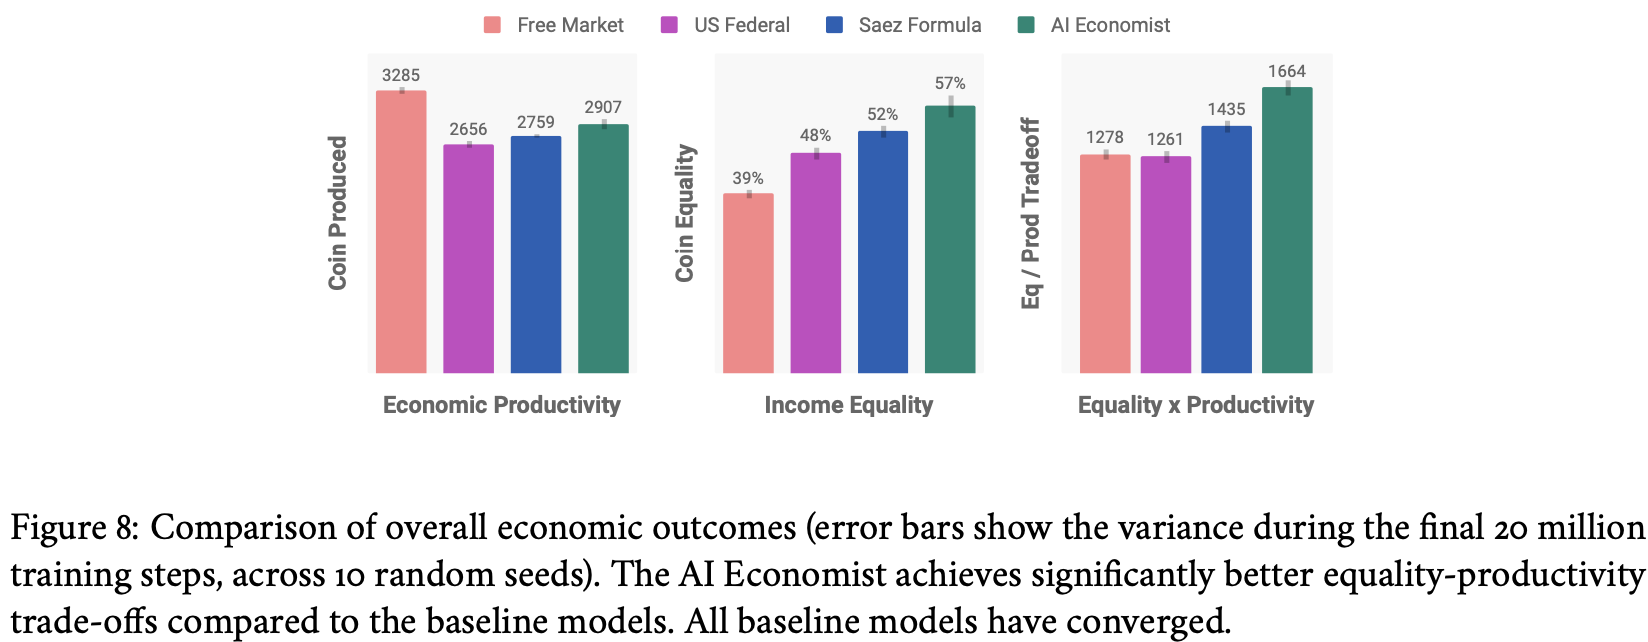
\includegraphics[width=10cm]{figure8.png}
    \end{center}
    \begin{itemize}
        \item 1エピソード終了時の各税制での各指標の比較.
        \item 課税は常に生産性を下げるが, その下り幅はAI Economistが最も少ない.
        \item 平等性は, AI economistで最も高い.
        \item 社会厚生(平等性$\times$生産性)もAI economistが最も高く, 次に高いSaez formulaと比べても$16\%$高い.
    \end{itemize}
\end{frame}

\begin{frame}{}{}
    \begin{center}
        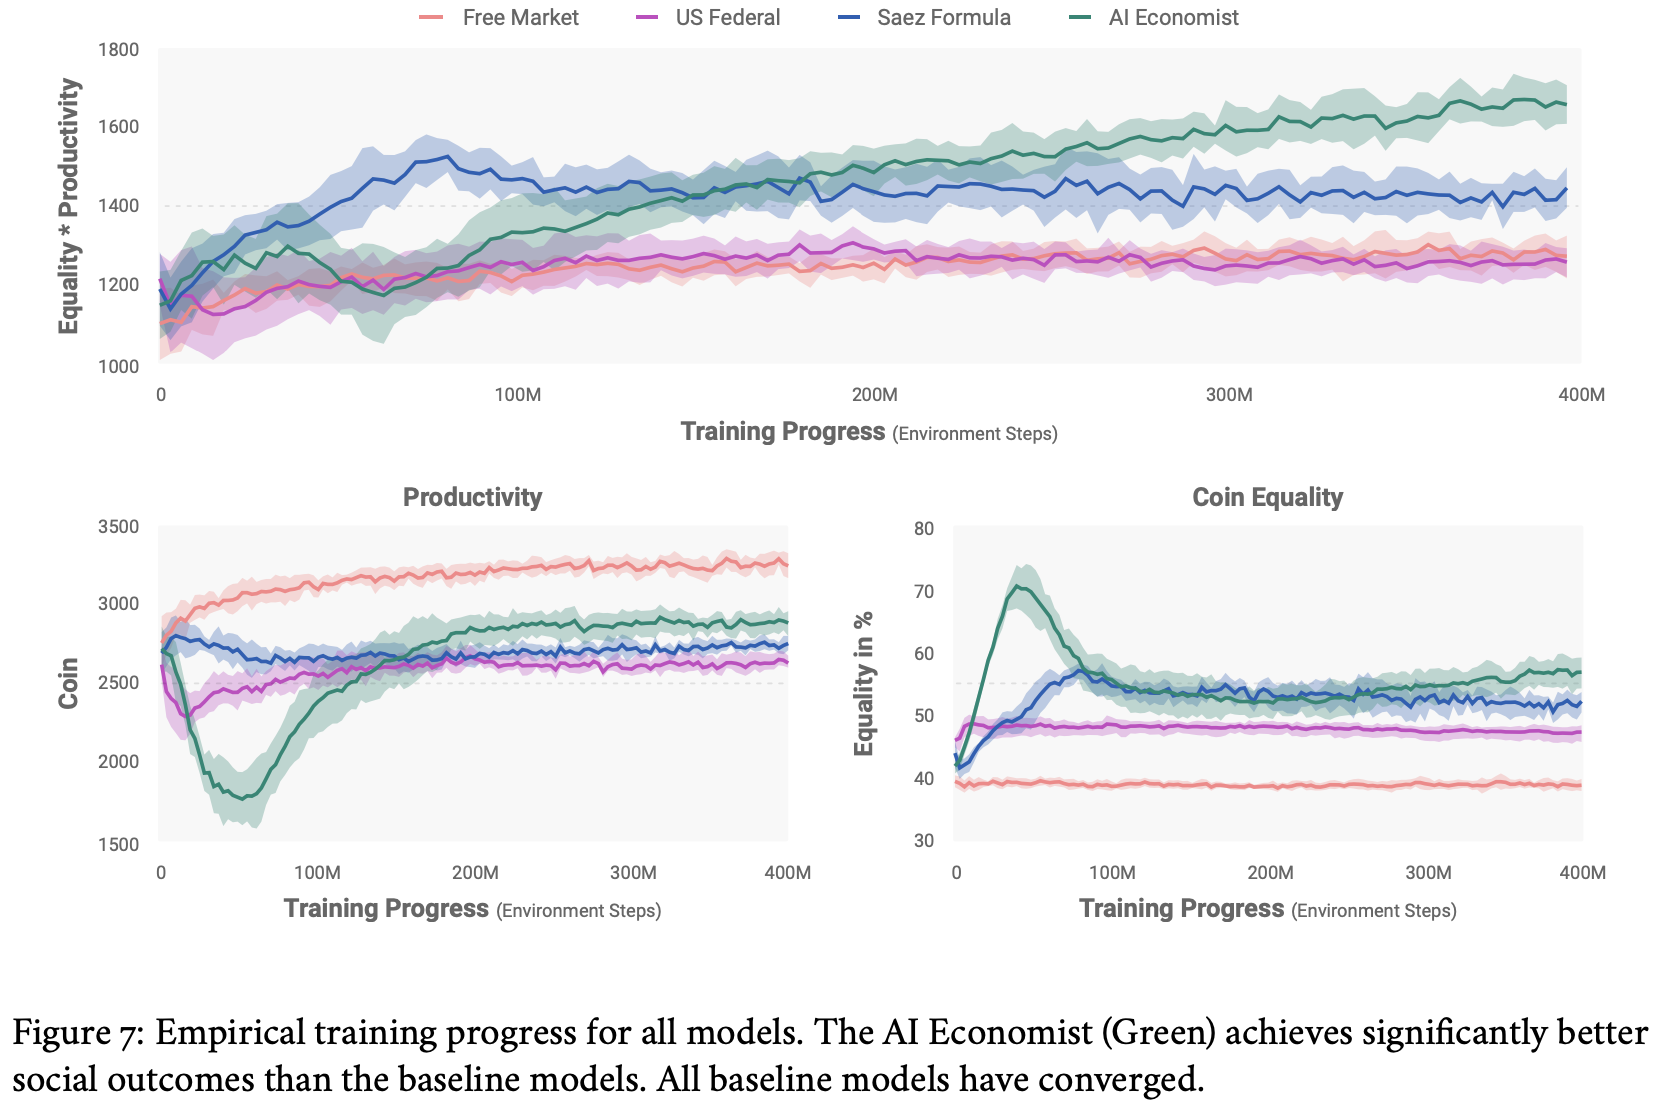
\includegraphics[width=12cm]{figure7.png}
    \end{center}
\end{frame}

\subsection{4.4 税額関数と課税額・再分配額の比較}
\begin{frame}{4.4 税額関数と課税額・再分配額の比較}{}
    {\bf 税額関数}
    \begin{columns}
        \begin{column}{0.5\textwidth}
            \begin{center}
                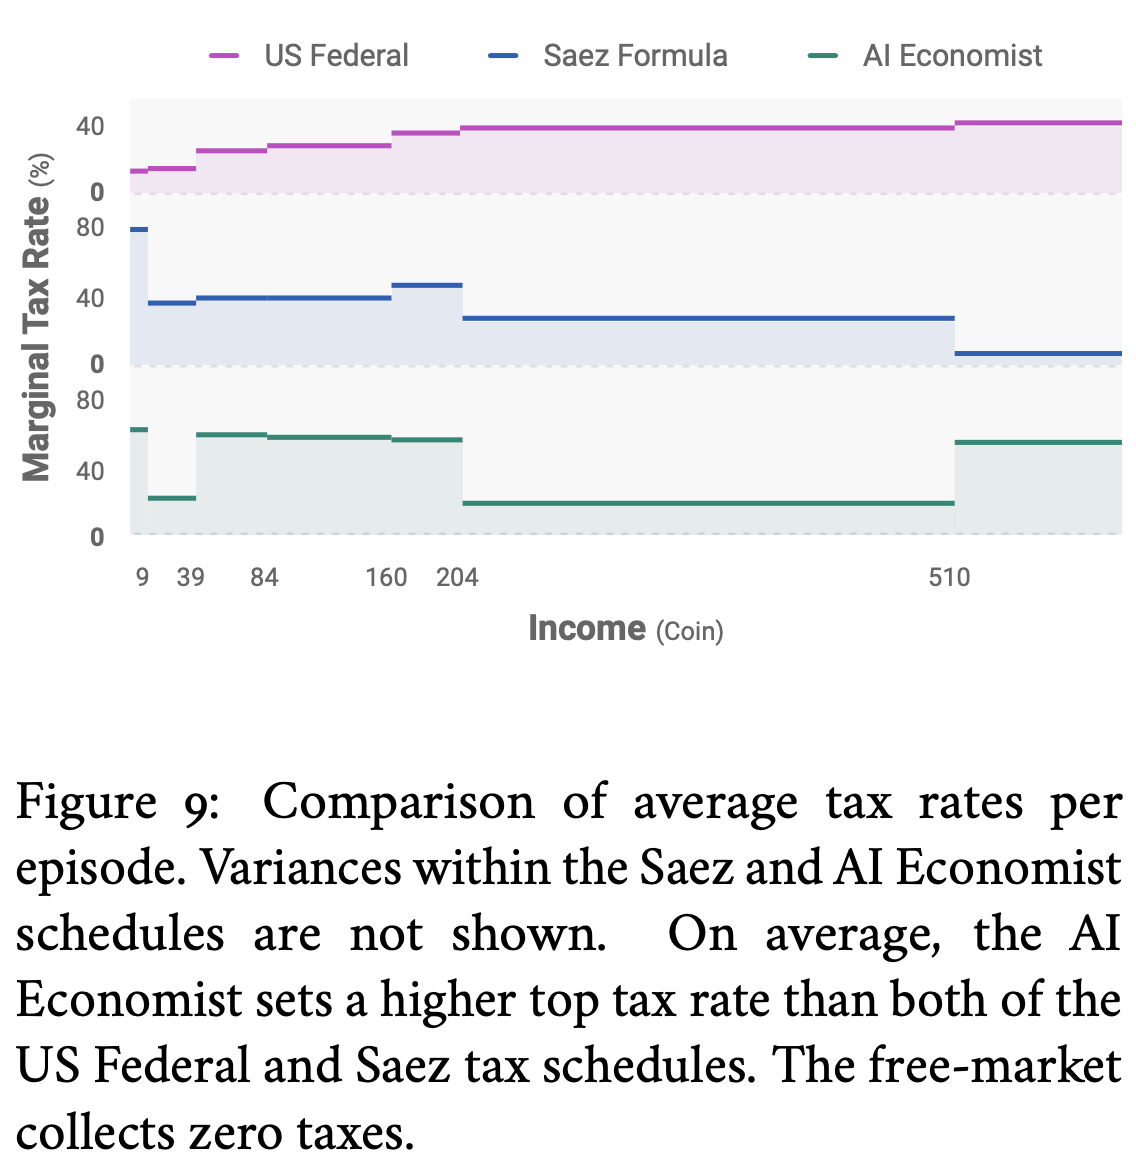
\includegraphics[width=6cm]{figure9.png}
            \end{center}
        \end{column}
        \begin{column}{0.5\textwidth}
            \begin{itemize}
                \item 左図は各税制での限界税率の比較.
                \item 米所得税は高ブラケットに対して限界税率が上がっていく.
                \item Saez formulaでは概ね逆.
                \item AI Economistはそのブレンドになってる.
            \end{itemize}
        \end{column}
    \end{columns}
\end{frame}

\begin{frame}{}{}
    {\bf 収入・課税額・再分配.}
    \begin{center}
        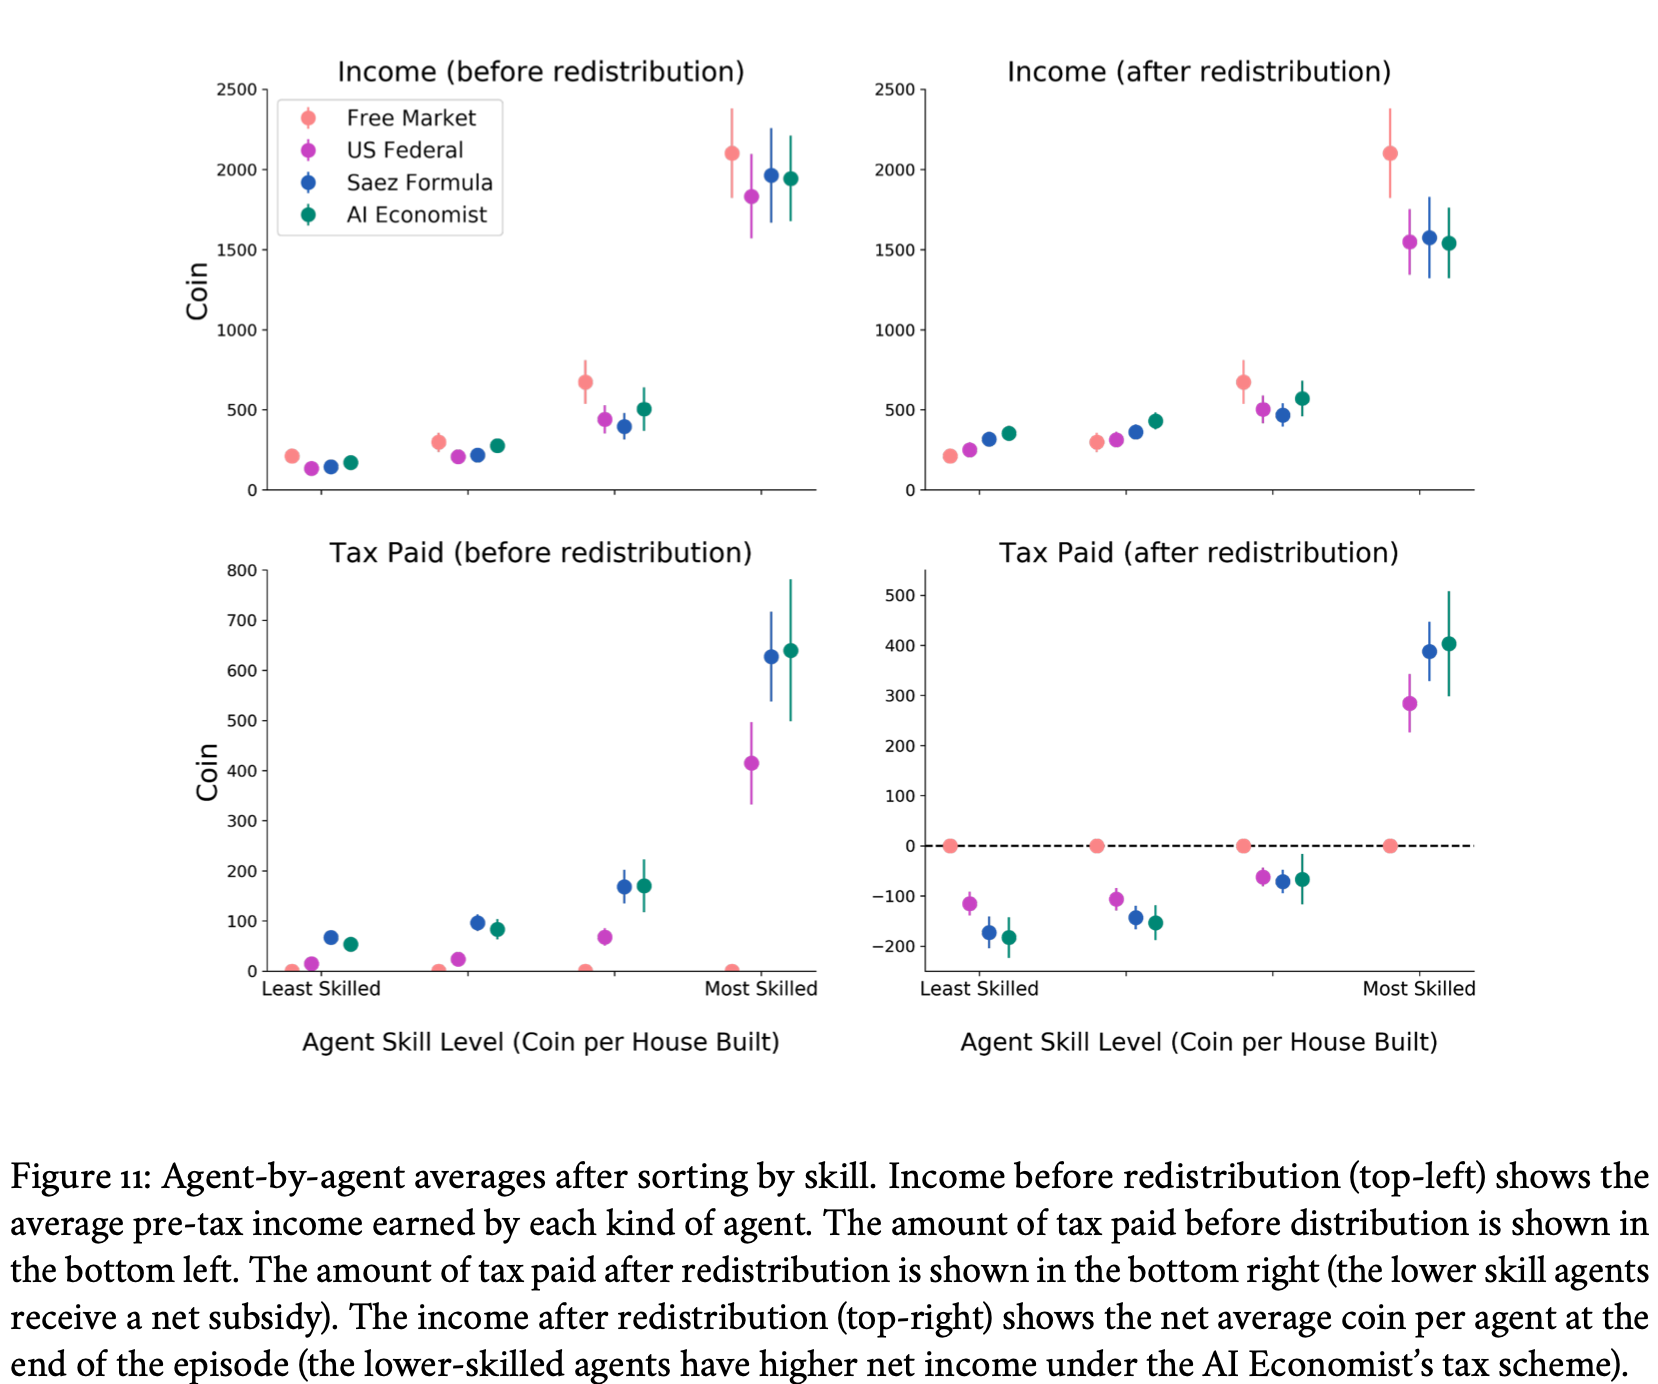
\includegraphics[width=10cm]{figure11.png}
    \end{center}
\end{frame}

\begin{frame}{}{}
{\bf 市民の行動への影響}
\begin{center}
    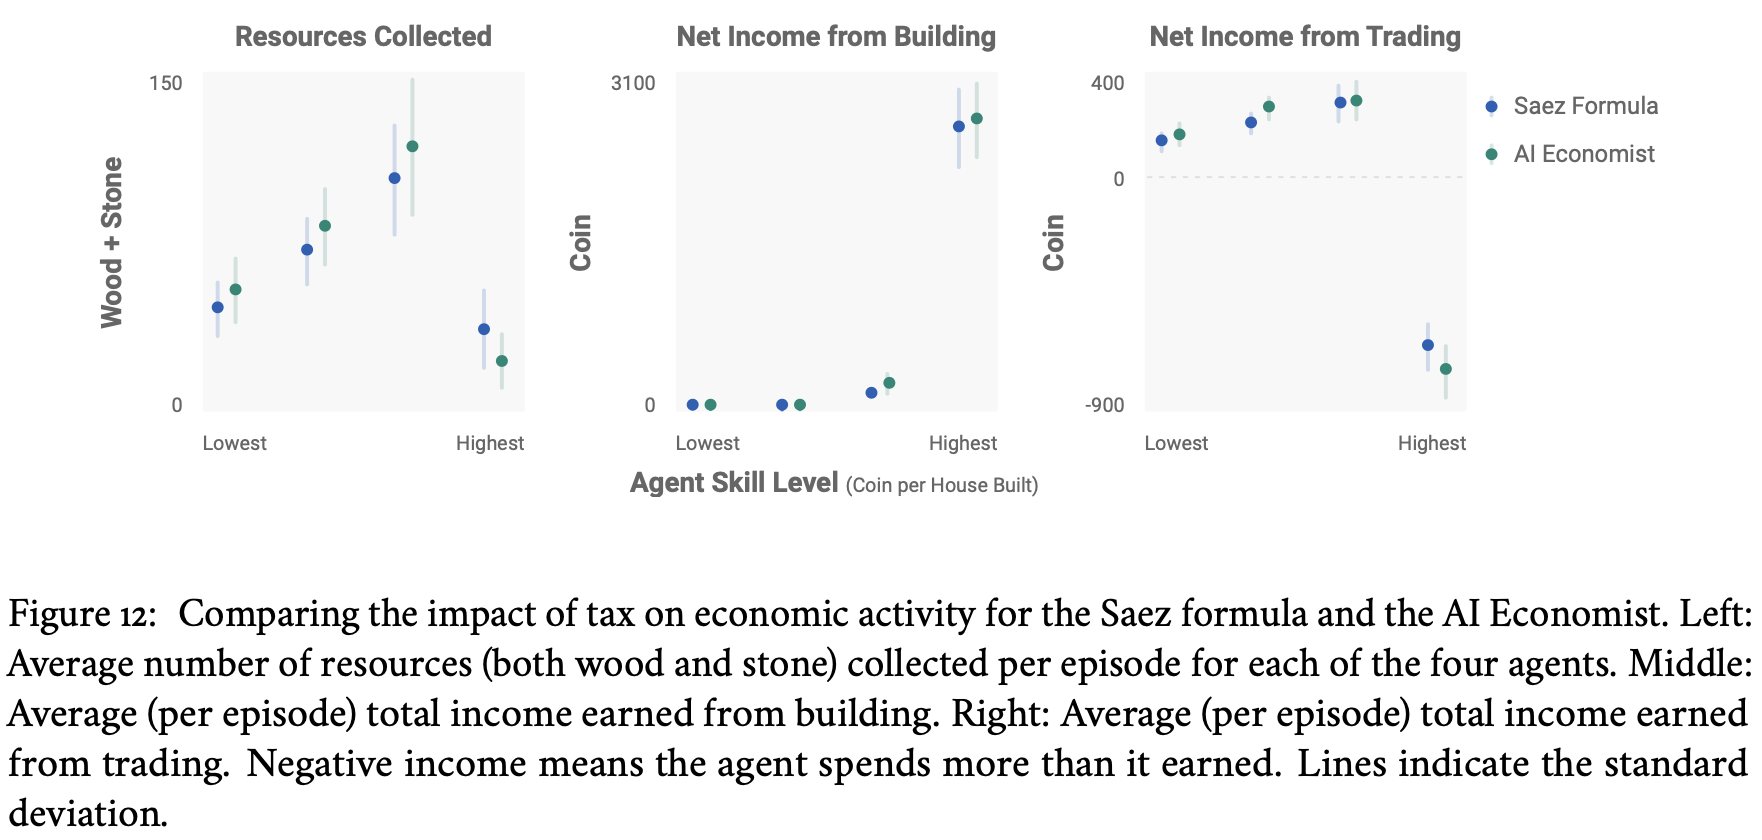
\includegraphics[width=10cm]{figure12.png}
\end{center}
\begin{itemize}
    \item 上手は, Saez frameworkとAI economistでの市民の行動の比較.
    \item AI economistでは, 高スキル市民は資源を集めるより, 市場で買って建築することに特化し, 低スキル市民はより資源を集めるようになっている.
\end{itemize}
\end{frame}

\begin{frame}{4.5 Tax-Gaming Strategies}{}
    \begin{center}
        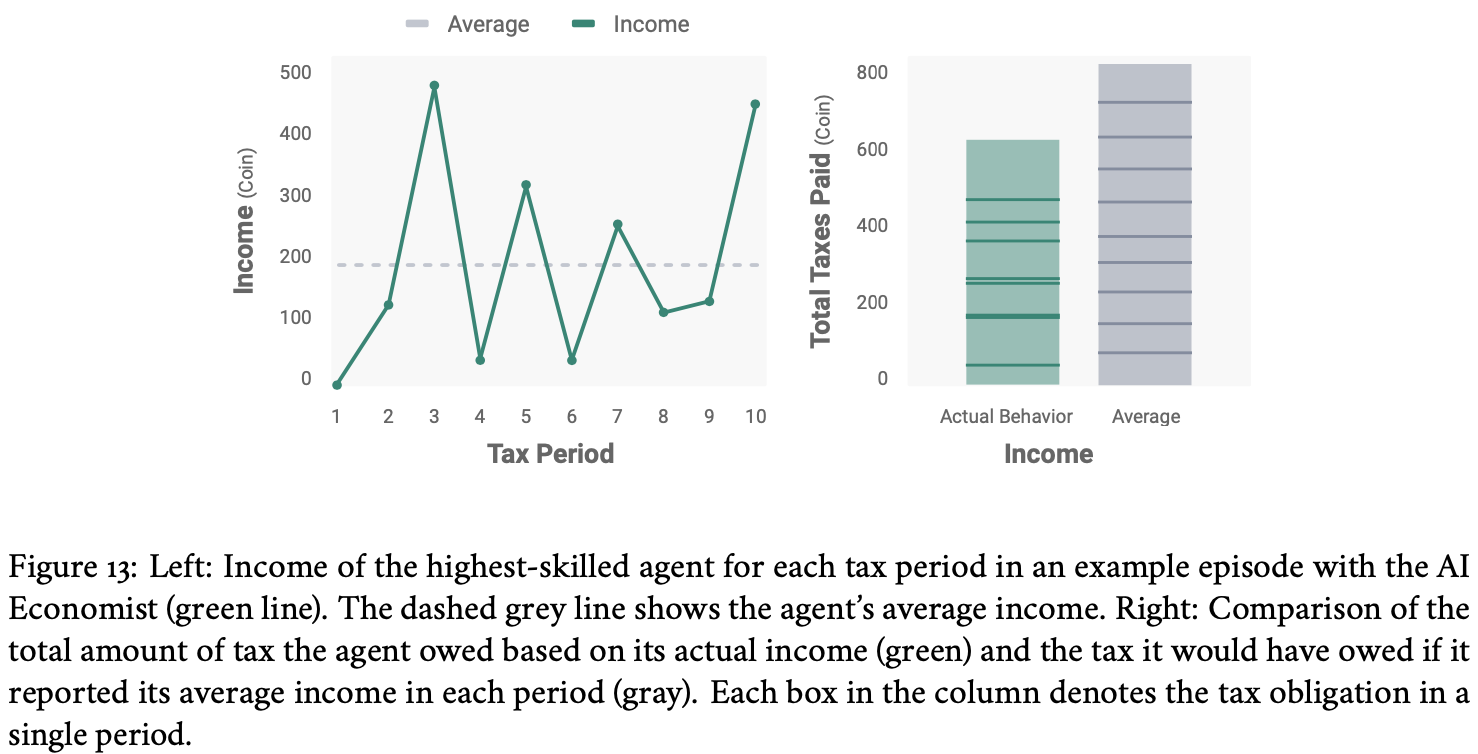
\includegraphics[width=11cm]{figure13.png}
    \end{center}
    {\footnotesize\begin{itemize}
        \item 上図はAI economistでの高スキル市民の1エピソード間の収入推移.
        \item 高収入の税ピリオドと低収入の税ピリオドが交互に起きている.
        \item 市民は収入をばらつかせることで課税額を抑えるように行動している(Saezでも同様)
    \end{itemize}}
\end{frame}

\section{5. 被験者実験}

\begin{frame}{5. 被験者実験}{}
    \begin{itemize}
        \item AI economistの税制が, 人間が参加する経済シミュレーションでも結果をよくするか検証する.
        \item Amazon Mechanical Turk (MTurk) platformにおいて実験を行った.
    \end{itemize}
\end{frame}

\begin{frame}{5.1 実験方法}{}
    \begin{itemize}
        \item 設定は基本的に同じだが, 若干の変更がある:
        \begin{itemize}
            \item 取引は行わないようにする.
            \item 労働コストがかかるのは建築のみとし, 移動・収集・取引は0コストとする. ただし建築の労働コストは$50\%$増し.
            \item 各エピソードは5分間で, フレーム率は1秒あたり10フレーム.
            \item 各エピソードは3000ステップ. 各税ピリオドは300ステップ.
        \end{itemize}
    \end{itemize}
\end{frame}

\begin{frame}{}{}
\begin{columns}
    \begin{column}{0.6\textwidth}
        {\bf 税制.}
        \begin{itemize}
            \item 税制もAI市民実験と基本的に同様.
            \item 無課税, 2018米所得税はそのまま.
            \item Saez formulaは, 学習後の1エピソード間の平均税率とする.
            \item AI economistは, AI実験から効果的だった1制度を1つ使った("Camelback"モデル)
        \end{itemize}
    \end{column}
    \begin{column}{0.4\textwidth}
         \\
        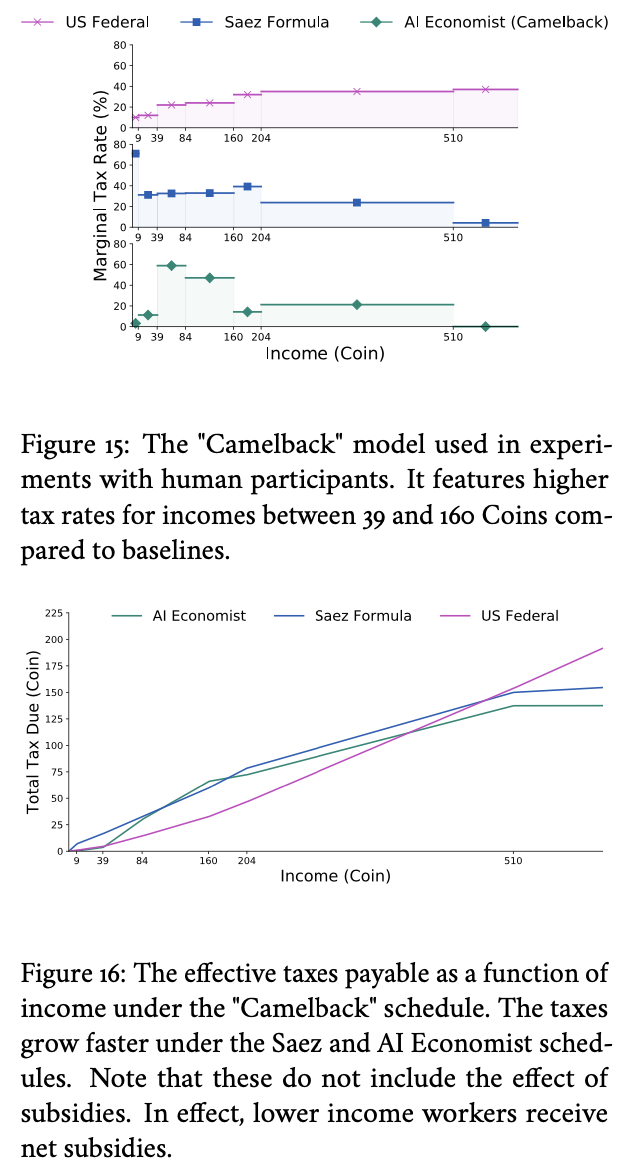
\includegraphics[width=4.7cm]{figure15.png}
    \end{column}
\end{columns}
\end{frame}

\begin{frame}{}{}
{\bf 支払い.}
\begin{itemize}
    \item 各参加者はベース報酬 $\$5$ とボーナス報酬最大 $\$10$ を得る.
    \item このボーナスは, \[\mathrm{USD\ bonus} = \mathrm{Utility}\times 0.06, \tag{26}\]で計算される.
    \item 平均の合計支払い額は, $\$ 11.26$ だった.
\end{itemize}
\end{frame}

\begin{frame}{5.2 結果}{}
    \begin{columns}
        \begin{column}{0.5\textwidth}
            {\bf 社会厚生の比較}
            \begin{itemize}
                \item 社会厚生(平等性$\times$生産性)は, AI economistの結果は米所得税, Saezフレームワークと比べて悪くなく, 無課税より有意に高かった.
                \item おおむねAI egentsでの実験と同等の結果.
            \end{itemize}
        \end{column}
        \begin{column}{0.5\textwidth}
            \begin{center}
                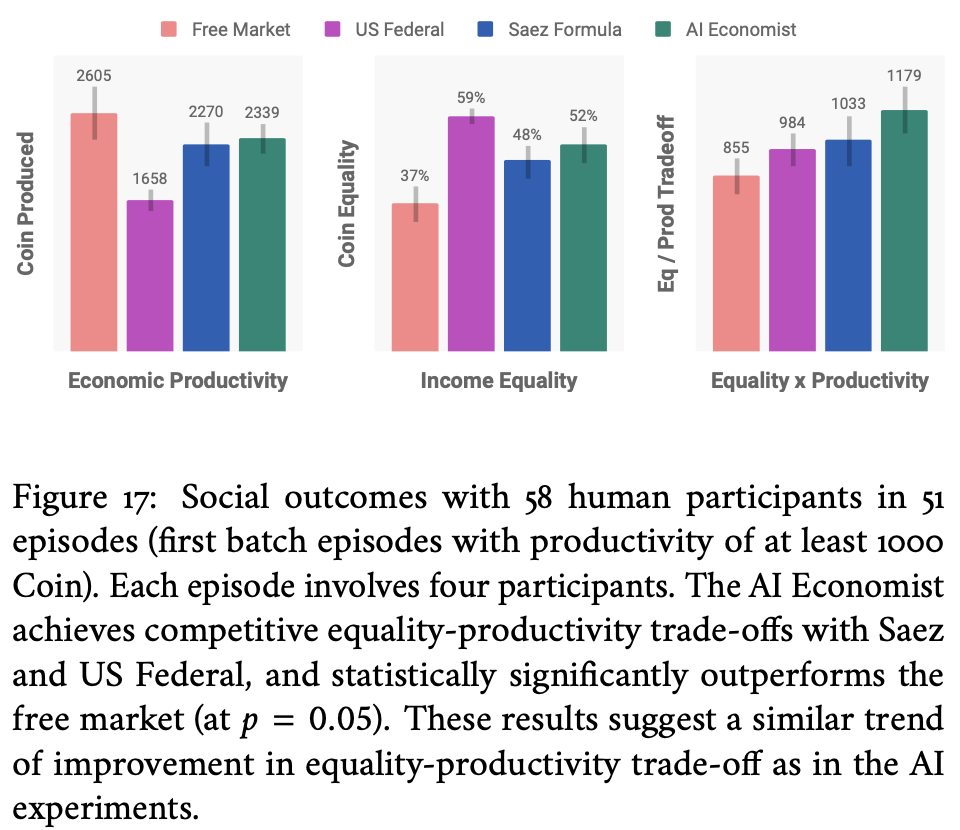
\includegraphics[width=7cm]{figure17.png}
            \end{center}
        \end{column}
    \end{columns}
\end{frame}

% \begin{frame}{}{}
%     \begin{columns}
%         \begin{column}{0.6\textwidth}
%             \begin{itemize}
%                 \item Inverse post-tax endowmentsをweightとしたsocial welfare functionも評価した:
%                 \[
%                     {\bf swf}_{H}(\bm{x}_H^c, \bm{l}_H) = \sum_{i=1}^N \omega_i \cdot u_i\left(x_{i,H}^c, l_{i,H}\right), \tag{27}
%                 \]
%                 where
%                 \[\omega_i = \frac{\tilde{\omega}_i}{\sum_j \tilde{\omega}_j},
%                 \ \ \ \tilde{\omega}_i = \frac{1}{x^c_{i, H}}.\]
%                 \item AI economistは他の全てのbaselineより有意に高かった.
%             \end{itemize}
%         \end{column}
%         \begin{column}{0.4\textwidth}
%             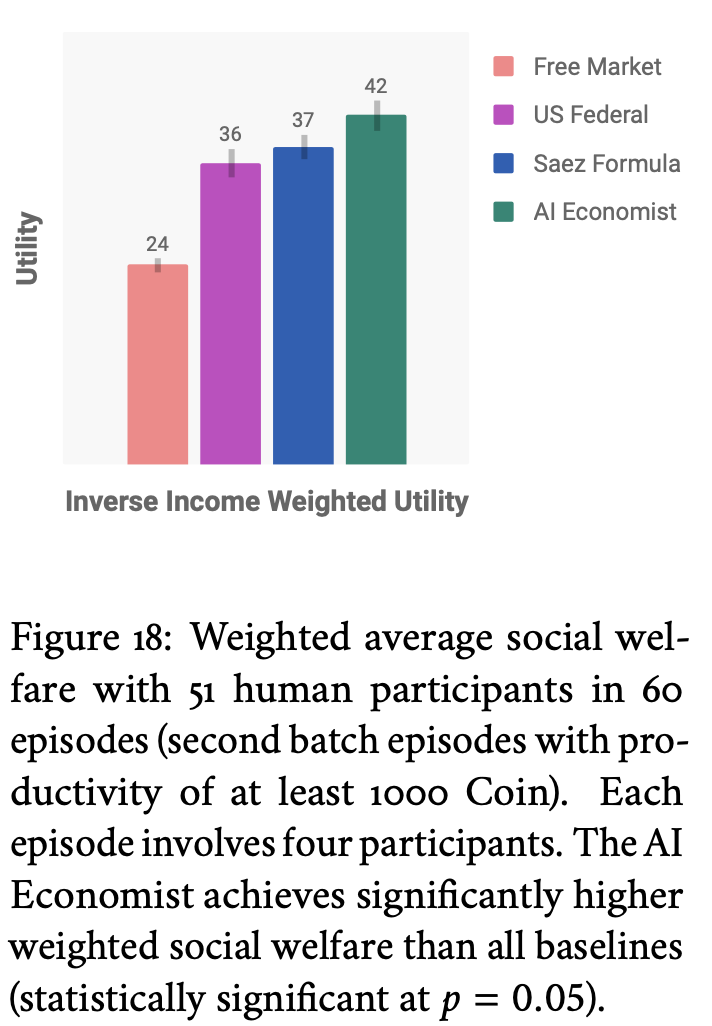
\includegraphics[width=6cm]{figure18.png}
%         \end{column}
%     \end{columns}
% \end{frame}

\section{6. 結論}

\begin{frame}{6. 結論}{}
    \begin{itemize}
        \item 生産性と平等性のトレードオフを上手くバランスする最適な税制を求めることは重要だが難しい.
        \item 経済シミュレーションにおいて, 深層強化学習を用いて政府主体に最適な税制を学習させることが考えられた.
        \item AI市民と被験者による実験の双方で, Ai economistはベースライン税制(無課税・米所得税・Saezフレームワーク)と比較して高い水準の社会厚生を達成した.
    \end{itemize}
\end{frame}
\end{document}
